%% ---------------------------------------------------------------------------%
%% main.tex - Part 3 Project Final Report, Ricardo da Silva
%% tab_size: 2
%% ---------------------------------------------------------------------------%
% Preamble
\documentclass{ecsproject}     			% Use the ECS Project Style
\usepackage[square,numbers]{natbib}	% Use Natbib style for the refs.
\graphicspath{{../Figures-Final/}}  % Location of figures
\hypersetup{colorlinks=true}				% Set to false for b/w printing
\setboolean{@twoside}{false}				% Set true for a page gutter

\usepackage[disable]{todonotes}  		% Possible option: disable
\newcommand{\inote}[1]{\todo[inline]{#1}}  % type \inote{bla bla}

\usepackage[titletoc]{appendix}     % Put 'Appendix' in TOC
\usepackage{array}

%\begin{document}
def
\end{document}                % Include abbreviations
\usepackage[intoc]{nomencl}					% Use the nomenclature package
\makenomenclature % TODO: run `makeindex Main.nlo -s nomencl.ist -o Main.nls`
\renewcommand{\nomname}{Nomenclature and Abbreviations}

\newcommand{\meq}[2] {							% Equation macro. \meq{label}{math}
	\begin{align} \label{eq:#1} #2
	\end{align}
}

\newcommand{\dobib}[1] {
  \if@openright
    \cleardoublepage
  \else
    \clearpage
  \fi
  \addtotoc{\bibname}
  \bibliography{#1}
}

\lstdefinestyle{customc}{						% Custom C listing style
  belowcaptionskip=1\baselineskip,
  breaklines=true,
  frame=L,
  xleftmargin=\parindent,
  language=C,
  showstringspaces=false,
  %basicstyle=\footnotesize\ttfamily,
  keywordstyle=\bfseries\color{green!40!black},    % Comment out for b/w
  commentstyle=\itshape\color{purple!40!black},
  identifierstyle=\color{blue},
  stringstyle=\color{orange},
}

\def\figwidth{0.8\textwidth}    % Figure width used for most figures

\renewcommand{\arraystretch}{1.3}  % Increase row separation in tables

%\includeonly{,,} % Only compile these files
%% ---------------------------------------------------------------------------%
\begin{document}
\frontmatter
\title      {Speech Recognition on Embedded Hardware}
\authors    {\texorpdfstring
             {\href{mailto:rmds1g10@ecs.soton.ac.uk}{Ricardo da Silva}}
             {Ricardo da Silva}
            }
\addresses  {\groupname\\\deptname\\\univname}
\date       {April, 2013} % {\today}
\subject    {}
\keywords   {}
\supervisor {Dr Steve Gunn}
\examiner   {Dr Nick Harris}
\degree     {Electronic Engineering with Mobile and Secure Systems} %TODO fix
\maketitle
\begin{abstract}  % 141 words
% the Abstract summarises the purpose of the project and what was achieved by the project.
This report presents a proof of concept system that is aimed at investigating Hidden Markov Model based speech recognition in embedded hardware.  It makes use of two new electronic boards, based on a Spartan 3 FPGA and an ARMv5 Linux applications processor, that are currently under development at the University of Southampton.  Speech data is pre-processed in Linux, by performing spectral analysis followed by a Discrete Cosine transformed filter-bank analysis, to produce Mel Frequency Cepstral Coefficients.  Given this observation data, the FPGA performs the most computationally intensive part of a modern HMM based speech recognition system -- evaluating the state emission probabilities.  It is shown that the FPGA is capable of performing these calculations faster than a software implementation on the Linux processor.  The resulting system is also a valuable example of how these two boards may be used in a practical setting.
\end{abstract}
\tableofcontents
\listoffigures
%\listoftables
%\lstlistoflistings
%\listofsymbols{ll}{$w$ & The weight vector}
\acknowledgements{Thanks to Steve Gunn, Srinandan Dasmahapatra}
\authorshipdeclaration{Ricardo da Silva}
%\dedicatory{To \dots}
\clearpage
\markboth{\nomname}{\nomname}
\printnomenclature
\cleardoublepage
%% ---------------------------------------------------------------------------%
% See https://cs.uwaterloo.ca/~brecht/thesis-hints.html
\mainmatter

%!TEX root = Main.tex
% Introduction: words
\chapter{Introduction} % (fold)
\label{cha:introduction}

% Introduce the project, talk about the planned and final goals, my contribution, what I learnt, and a short conclusion.
% Make it clear that it's a POC system

\section{Goals} % (fold)
\label{sec:goals}
	At the highest level, the primary goal of this project is to implement part of a modern HMM based speech recognition system, with the constraint that it must be done on embedded hardware.  In pursuing this goal, the aim is to achieve several other goals that will be beneficial to the author and to the University of Southampton.

	\subsection{Speech Recognition} % (fold)
	\label{sec:speech_recognition}
		A complete HMM based speech recognition system is extremely complex, and can take years to design and optimise for a particular implementation.  The goal of this project is not to implement one such system, but rather to explore the possibilities of what may be achieved with a low power applications processor and a relatively small FPGA.  In particular, the goal is to use the applications processor (running Linux) to perform pre-processing of speech data, and use the FPGA to perform mathematical manipulations of the observations.  It is hoped that the system developed here may be later used as a basis for future research into the subject.
	% subsection speech_recognition (end)

	\subsection{The Micro Arcana} % (fold)
	\label{sec:the_micro_arcana}
		The Micro Arcana is a new hardware platform aimed at undergraduate students, currently under development by Dr Steve Gunn.  
		In terms of hardware, one of the project goals is to further development of the Micro Arcana family of boards, and provide a valuable use case example as described in the Motivation section.  Part of the project is setting up and configuring these two boards, so that they may be easily picked up by undergraduates.  In addition, the aim is to build the entire system on these two boards, making it a self-contained embedded design and showing how they may be usefully combined.
	% subsection the_micro_arcana (end)

	\subsection{Theoretical understanding} % (fold)
	\label{sec:theoretical_understanding}
		A major goal of the project is to develop a higher level of understanding of the algorithms used in speech recognition, and to get experience designing a large-scale embedded application.  This complements the interests of the author and the subjects being studied, in particular, Intelligent Algorithms and Digital Systems Design.
	% subsection theoretical_understanding (end)

% section goals (end)

\section{Motivation} % (fold)
\label{sec:motivation}
	Speech recognition is an interesting computational problem, for which there is no fool-proof solution at this time.  Recently the industry for embedded devices and small-scale digital systems has expanded greatly, but in general these devices do not have the power or speed to run speech recognition.  Field Programmable Gate Arrays (FPGAs) may present a way of increasing the capability of such systems, as they are able to perform calculations much faster than traditional microprocessors.  The author's personal interest in embedded systems, combined with the challenges of a complex system such as speech recognition, makes this an appealing area to explore.

	As hardware platforms go, most of the Micro Arcana is still very new and untested, as it is still under development.  In addition, there are not many examples of how they may be used, and very little documentation.  In order to improve their reception by students, it would greatly help to have proven use cases and examples of how these boards may be used individually and together.  Using a larger FPGA (such as an Altera DE board) was considered during the planning stages of this project, but it was decided that part of the challenge was to develop and use the Micro Arcana.
% section motivation (end)

\section{Contributions} % (fold)
\label{sec:contributions}
	The project implements one part of a modern speech recognition system, using two development boards from the Micro Arcana family.  It is designed to be a proof of concept exercise, in order to explore the capabilities of the boards, and expand the author's knowledge of the relevant systems.  Specifically, the project required substantial research into HMM based speech recognition systems, embedded Linux, and digital design.  The resulting system, described in detail in Chapter~\ref{cha:system_design}, uses an FPGA to perform the most computationally expensive part of HMM based recognisers -- scoring the states of each HMM model for a given input vector.  Essentially, the ARM based ``L'Imperatrice'' is used as the application controller, and is connected to the FPGA based ``La Papessa'' board which performs the CPU intensive mathematical calculations.  Given an observation vector, the FPGA will process it and send back scores for each state in the speech model.  The other main processes in a speech recogniser, such as pre-processing and decoding, are tasks that are well suited to software implementation.

	% TODO
	% Why is this useful?
	% What did I have to learn to accomplish this? 
% section contributions (end)


% chapter introduction (end)
    % Mostly done
%!TEX root = main.tex
% 1265 words
\chapter{Background and Investigations} % (fold)
\label{cha:background}

\section{Speech Recognition Systems} % (fold)
\label{sec:speech_recognition_systems}
In general, `Speech Recognition' refers to the process of translating spoken words or phrases into a form that can be understood by an electronic system, which usually means using mathematical models and methods to process and then decode the sound signal.  Translating a speech waveform into this form typically requires three main steps \cite{melnikoff2003speech}.  The raw waveform must be converted into an `observation vector', which is a set of data that is compatible with the chosen speech model.  This data is then sent through a decoder, which attempts to recognise which words or sub-word units were spoken.  These are then sent through a language model, which imposes rules on what combinations of words of syntax are allowed.  This project aims to focus on the first and second tasks, as they are the more interesting from an electronic engineering point of view.

There are a variety of different methods and models that have been used to perform speech recognition.  An overview of the most popular will be described here, along with the chosen approach.

\subsection{Tor's Algorithm} % (fold)
\label{sub:tors_algorithm}
The author first became interested in speech recognition when reading about ``Tor's Algorithm'', which is a very simple small dictionary speech recognition system \cite{tor2003}.  This algorithm is capable of very accurate speaker dependent speech recognition for a dictionary of less than ten words.  It is based on a fingerprinting model where each word in the dictionary must be trained to form an acoustic `fingerprint'.  This fingerprint is based on the time variations of the speech signal after being filtered appropriately.  Then recognition is reduced to finding the Euclidean distance squared between the input vector and each of the stored fingerprints.  The `closest' match is the word with the smallest distance from the input.
Although this system is very simplistic, it outlines two major components of any speech recognition system -- pre-processing and decoding (recognition).  More complex systems just use more complex speech models and pre-processing methods.
% subsection tors_algorithm (end)

\subsection{Dynamic Time Warping} % (fold)
\label{sub:dynamic_time_warping}
Speech, by nature, is not constrained to be at a certain speed -- the duration of words will vary between utterance, and a speech recognition system should be able to handle this.  Dynamic Time Warping (DTW) is essentially the process of expanding and contracting the time axis, so that waveforms may be compared, independent of talking speed.  Combined with a dynamic programming technique for finding the optimal `warp' amount, it became a widely used approach to solving the problem of speech duration modelling \cite{furui1989speech}.  One useful property of DTW is that it may offer good performance even with little training, as it only needs one word as a template \cite{melnikoff2003speech}.  Conversly, the performance of DTW based systems cannot be increased much with more training, unlike Hidden Markov Models.
% subsection dynamic_time_warping (end)

\subsection{HMMs} % (fold)
\label{sub:about_hmms}
By far the most prevalent and successful approach to modern speech recognition uses Hidden Markov Models (HMMs) for the statistical modelling and decoding of speech \cite{cox1988hidden}.  The flexibility inherent in HMMs is key to their success, as a system can be made more and more accurate by simply improving the HMM models or training the models further.  The classic tutorial paper by Rabiner (\cite{rabiner1989tutorial}) is one of the best references for HMMs in speech recognition, and provides a very good overview of modern systems.  The following three sections are based heavily on \cite{rabiner1989tutorial} and \cite{htkbook}.

% \subsubsection{Single Word HMMs} % (fold)
% \label{ssub:single_word_hmms}
The simplest HMM based systems use a single HMM for every word in the recognition dictionary.  Given a set of observations, each HMM can be scored based on the probability that it would output the observations.  The HMM with the highest score is taken as the recognised word.  The most apparent limitation of this system is that a very large amount of training would be required if a dictionary of any size was to be used.  At the very least, one sample of each word would need to be recorded to train the full system, which would be a very time consuming process.  However, for simple applications (voice dialling, for example) this is manageable.
% subsubsection single_word_hmms (end)

% \subsubsection{Sub-word HMMs} % (fold)
% \label{ssub:sub_word_hmms}
The next step up in complexity from single word HMMs is models that consider sub-word utterances (phonemes).  This allows a smaller set of HMMs to be used for much larger dictionary recognition, as words are recognised based on sequences of sub-word HMMs.  Thus instead of searching through a single HMM to recognise a word, the recognition process becomes a search through a trellis of multiple HMMs in order to find the best path through them.  The most simple HMM system of this form is based on mono-phones, of which there are about 50 in English.  This may be improved by using bi- or tri-phone HMMs, which model transitions between two or three mono-phones.  Using this form of HMM will increase the acoustic model size greatly however, as there are many possible combinations of mono-phones in the English language.
% subsubsection sub_word_hmms (end)

% \subsubsection{Viterbi Decoding} % (fold)
% \label{ssub:viterbi_decoding}
For most HMM models there are three problems: 
\begin{itemize}
	\item Training the model
	\item Finding the probability that a model produced a given observation sequence
	\item Finding the `best' path through a model to produce a given observation sequence
\end{itemize}
The `best' path is generally taken to be the path with highest probability, and it is this problem that is central to the project.  The first problem is solved by using Voxforge (\ref{sec:the_htk}), and the second problem is more important for word based recognisers.

In all literature encountered, the Viterbi algorithm is the primary method for solving problem 3.  It is an iterative approach to solving the optimisation problem, and has the added bonus that not much data needs to be stored during the calculation \cite{schuster2006speech}.  A full explanation of the Viterbi decoding process is available from \cite{rabiner1989tutorial},\cite{melnikoff2003speech},\cite{saeed2008advanced}.
% subsubsection viterbi_decoding (end)

% subsection about_hmms (end)
% section speech_recognition_systems (end)


\section{Speech Pre-Processing} % (fold)
\label{sec:speech_pre_processing}
Speech signals are complex waveforms and cannot be processed without some form of feature extraction which reduces the complexity while retaining the important features.  In modern speech recognition systems the two most common methods of analysing and representing speech are: \cite{gaikwad2010review}
\begin{itemize}
	\item Linear Predictive Coding (LPC)
	\item Mel-Frequency Cepstrum Coefficients (MFCC)
\end{itemize}
Both these methods attempt to model the movement and dynamics of the human vocal tract and auditory perception.  LPC is more suited to speaker recognition (the process of identifying voices, rather than speech), while MFCCs are more useful for speech recognition \cite{sd2012interview}.

The Mel-Frequency Cepstrum is based on a filterbank analysis with a cepstral transformation, which is required due to the high correlation between filterbank amplitudes.  The human ear perceives sound on a non-linear frequency scale, and one way of improving recognition performance is by using a similar scale for analysis of speech.  A filterbank analysis can be used to perform this discrimination between different frequencies, and the frequency bins are usually spaced using the Mel frequency scale.  However, the filterbank amplitudes are highly correlated, which greatly increases the computational complexity of the HMM based recogniser as the covariance matrix will not be diagonal.  In order to correct this, a discrete cosine transform is taken on the log filterbank amplitudes, finally resulting in a set of Mel Frequency Cepstrum Coefficients.  The HTK (\ref{sec:the_htk}) defaults to using twelve MFCC filterbank bins. \cite{htkbook} \cite{melnikoff2003speech}

In order to attain MFCCs, a sampling rate must be chosen such that enough data is gathered while allowing sufficient processing time.  In addition, to perform Fourier transforms on the speech, the incoming signal must be windowed appropriately.  The HTK has a set of default values for these parameters, which are assumed to be appropriate.

An improvement to both LPC and MFCCs is to compute time derivatives in the feature extraction process, which gives a better idea of how the signal changes over time.  In addition, the log energy of each sample may also be computed to also boost recognition ability.

% section speech_pre_processing (end)


\section{The HTK and VoxForge} % (fold)
\label{sec:the_htk}
The Hidden Markov Model Toolkit (HTK) is a set of tools and libraries for developing and testing Hidden Markov Models (HMMs), primarily for speech processing and recognition tools \cite{htkbook}.  Given a model structure and a set of transcribed speech recordings (a `speech corpus'), a set of HMMs may be trained using the HTK.  This includes performing all pre-processing in a number of formats, and testing recognition capabilities of a model.

Voxforge is an open source speech corpus which is aimed at facilitating speech recognition development.  It provides pre-compiled acoustic models -- essentially large sets of HMMs -- in the format created by HTK, licensed under the GPL (GNU General Public License) \cite{voxforge}.  The alternative would be to use another speech corpus (such as TIMIT), and then use the HTK to design and train the acoustic model.  This is potentially a very time consuming process, so Voxforge is useful because it essentially cuts this step out.  In addition, the Voxforge models may be easily adapted to a specific person's voice using only a few minutes of transcribed speech.  However, the drawback is that the Voxforge model is very complex (~8000 tri-phone HMMs with Gaussian output probabilities, 25 coefficient observation vectors).  Implementing a recogniser system based on this model will require a lot more work than if a simpler model was used, such as one based on discrete (output probability) HMMs.
% section the_htk (end)


\section{Embedded hardware and Speech Silicon} % (fold)
\label{sec:embedded_hardware}
A wide range of speech recognition software (commercial and open source) exists for desktop PCs or laptops.  However, speech recognition for embedded systems is less widespread.  Recently there has been increased research into the use of DSPs and FPGAs for speech recognition \cite{melnikoff2003speech}, \cite{schuster2006speech}, \cite{nedevschi2005hardware}.  Of particular interest is Stephen Melnikoff's PhD Thesis, and the Speech Silicon architecture.  The former investigates a variety of HMM based recognisers on an FPGA, using a PC to perform pre and post processing.  The latter details a flexible FPGA based system capable of performing recognition on medium-sized vocabularies.
% section embedded_hardware (end)


% chapter background (end)      % Partially.  Needs expansion on FPGA stuff
%!TEX root = Main.tex
% Design Approach: words
\chapter{Design Theory and Approach} % (fold)
\label{cha:design_approach}

% TODO: What does this chapter give the reader??
%   All the main theory behind the approach
%   A description of what will be done

This chapter provides details of the relevant theory behind HMM based speech recognition systems, as well as a description of the various development environments used during the project.

\section{The HMM based model} % (fold)
\label{sec:the_hmm_based_model}
	Due to the flexibility of HMMs, and the complexity of speech, there have been several different approaches to building speech models (the sheer size of the HTK book indicates how much flexibility exists).  However, at this stage, the implementation of these algorithms is a more interesting pursuit, rather than devising the best way of modelling speech.  Therefore, it was decided to use the pre-designed models from Voxforge for this project, and build the hardware to work with these models.  Thus, various parameters were fixed from the start, including:

	\begin{itemize}
		\item Sampling rate of audio: 8kHz. %(Low Pass Filter with $\omega_0 = 4kHz$ required).
		\item Window size: 25ms (duration of observation frames).
		\item Frame period: 10ms (time between observation frames).
		\item Pre-processing output: 12 MFCCs, 12 MFCC derivatives, 1 Energy measure.
		\item Output probabilities of HMM states: Single Gaussian distribution, 25-element mean and variance vectors.
		\item Number of monophones: 51 (Includes a monophone for silence.  This is also the number of transition matrices).
		\item Number of senones: \about7000.
		\item Number of HMMs: \about8300\footnote{There are more HMMs than senones because some senones are used in more than one HMM} (each with 3 outputting states).
	\end{itemize}

	The only modification made to the Voxforge models was that they were adapted for the author's voice, primarily to gain confidence with using the HTK and HMMs.  Please see Appendix~\ref{apdx:voxforge} for the scripts and HTK configuration files used to generate these models.

	The term `outputting states' refers to states that produce an observation -- most of the HMMs have 5 states in total, but the first and last are non-emitting.  The transition probabilities between states one and two, and between states four and five, are primarily used to model inter-HMM probabilities for decoding purposes.  The senones are context dependent, that is, there are many different senones for each monophone, each with different predecessor and successor monophones.

	\subsection{The HMM tasks} % (fold)
	\label{sub:the_hmm_tasks}
		For an HMM model, denoted as $\lambda$, there are usually three important problems: 
		\begin{itemize}
			\item Design and train the model to accurately represent real data -- adjusting $\lambda$ to maximise $P(O | \lambda)$.
			\item Finding the probability that an HMM produced a given observation sequence, $P(O | \lambda)$.
			\item Finding the `best' path through a trellis of HMMs and states to produce a given observation sequence.
		\end{itemize}
		For this project, the first problem is solved by using Voxforge (Section~\ref{sec:the_htk}).  The second problem is potentially very computationally expensive, as the speech model may be complex or large.  In particular, this step requires evaluating the output probability of each state in the model for every new observation frame, which is particularly time consuming if the HMMs have continuous output distributions.  In modern speech recognition systems, this step regularly accounts for up to 70\% of the total processing time \cite{lai2002performance}.  This is the step that the project focusses on.

		In all literature encountered, the Viterbi algorithm is the preferred method for solving the final problem.  It is an iterative approach to solving the optimisation problem, and has the added bonus that not much data needs to be stored during the calculation \cite{schuster2006speech}.  This problem is beyond the scope of the current project, but a full explanation of the Viterbi decoding process is available from \cite{rabiner1989tutorial}, \cite{saeed2008advanced}, \cite{young1989token}.
	% subsection the_hmm_tasks (end)

	\subsection{Senone scoring} % (fold)
	\label{sub:senone_scoring}
		As described in previous sections, the FPGA is to be used to compute HMM emission probabilities for every senone in the model, for every observation vector.  In this system the new vectors arrive once every 10ms, and there are about 7000 senones that must be evaluated.  The mathematical operations required to do this are now outlined. % TODO!!: some kind of 'this is x calculations'?

		If the observation vector at time $t$ is denoted as $\textbf{O}_t = {O_{t1}, O_{t2}, ..., O_{tN}}$, then the score of senone $j$ is $b_j(\textbf{O}_t)$ -- the probability of that senone producing $\textbf{O}_t$.  The output probability of each senone is an $N$-dimensional multivariate Normal distribution, represented by $N$-element vectors of means $\mu_j$ and standard deviations $\sigma_j$.  Usually an $N\times N$ covariance matrix  would be required, but due to the statistical nature of Mel Frequency Cepstral Coefficients, this matrix is diagonal, and thus can be represented with $N$ elements.  Therefore the score is given by:
		\meq{score1}{
			b_j(\textbf{O}_t)
			&= \mathcal{N}_N(\textbf{O}_t; \boldsymbol{\mu}_j,\boldsymbol{\sigma}_j^2) \\
			&= \prod_{n=1}^{N} \frac{1}{\sigma_{jn} \sqrt{2\pi}} 
					\exp\left(- \frac{(O_{tn} - \mu_{jn})^2}{2\sigma_{jn}^2} \right)
		}

		However, hardware computation of this equation may be greatly simplified by taking logarithms of both sides, removing the need to evaluate exponentials:
		\[
		\ln(\mathcal{N}(\textbf{O}_t; \boldsymbol{\mu}_j,\boldsymbol{\sigma}_j^2))=
		\]
		\meq{score_ln}{
			\left[ -\frac{N}{2} \ln(2\pi) - \sum_{n=1}^N \ln(\sigma_{jn}) \right] -
			\sum_{n=1}^N
				(O_{tn} - \mu_{jn})^2
				\left[ \frac{1}{2\sigma_{jn}^2} \right]
		}

		Furthermore, the square bracketed terms in Equation~\ref{eq:score_ln} do not depend on the observation, and thus may be pre-computed.  The final equation is reduced to subtract, square, multiply, and accumulate:
		\meq{score_final}{
			\ln(\mathcal{N}(\textbf{O}_t; \boldsymbol{\mu}_j,\boldsymbol{\sigma}_j)) =
			K_j - \sum_{n=1}^N (O_{tn} - \mu_{jn})^2 \Omega_{jn}
		}

		Where the precomputed values are:
		\[ K_j = - \frac{N}{2} \ln(2\pi) - \sum_{n=1}^N \ln(\sigma_{jn}) \]
		\[ \Omega_{jn} = \frac{1}{2\sigma_{jn}^2} \]

		% Nomenclature
			\nomenclature{$\lambda(\pi,a,b)$}{A fully defined Hidden Markov Model}
			\nomenclature{$\pi$}{The set of initial state probabilities}
			\nomenclature{$a_{ij}$}{The probability of transitioning from state $i$ to state j}
			\nomenclature{$b_j(O)$}{The probability of state $j$ emitting observation $O$}

			\nomenclature{$\mu_j$}{N-dimensional vector of means for state $j$, indexed from 1 to N}
			\nomenclature{$\sigma_j$}{N-dimensional vector of standard deviations for state $j$, indexed from 1 to N}
			\nomenclature{$K_j$}{Pre-computed constant for state $j$}
			\nomenclature{$\Omega_j$}{N-dimensional vector of pre-computed scaling factors for state $j$}


	% subsection senone_scoring (end)
% section the_hmm_based_model (end)


\section{Hardware environment} % (fold)
\label{sec:hardware_dev_env}
	% Detail the compilation environment etc, which SD card does what...
	As the Micro Arcana is still under active development, part of the project involved setting up and testing the two boards that were used.

	\subsection{L'Imperatrice} % (fold)
	\label{sub:l_imperatrice_env}
		Several important features on the ARM-based L'Imperatrice board are still very untested, including parts essential to the project.  It is based on a Freescale iMX23 ARMv5 applications processor.  To be used for the project, the following items were required (in order of importance):
		\begin{itemize}
			\item Native or cross compiler setup
			\item Application UART functionality
			\item GPIO functionality  \nomenclature{GPIO}{General Purpose Input Output}
		\end{itemize}

		A Linux Target Image Builder (LTIB) \nomenclature{LTIB}{Linux Target Image Builder} environment, which is primarily used for setting up board support packages (BSP), was installed on an Ubuntu virtual machine.  It has been used to build and test various kernel configurations, and also includes full cross-compiler support for the board.  It essentially provides a platform on which software for L'Imperatrice may be developed and deployed.
		In addition to LTIB, the ArchLinux Build System (ABS) was investigated as a potential alternative to LTIB.  The primary advantage of the ABS is that only a small number of files need to be distributed, which, when run, will download and compile all dependencies of the build.  An ABS configuration exists for the Olinuxino, a Linux board also based on the Freescale iMX23, which may be tweaked to suit the L'Imperatrice.  However, due to lack of time and the relative ease of the LTIB setup, this was not explored.
	% subsection l_imperatrice_env (end)

	\subsection{La Papessa} % (fold)
	\label{sub:la_papessa_env}
		The Xilinx FPGA-based La Papessa board is also being actively developed, and some of its features have not been tested.  In order to facilitate the development of code on the La Papessa board, several combinations of software environments were explored.  The FPGA is a Xilinx Spartan XC3S50AN, which is compatible with the Xilinx ISE Webpack design software package.  However, one drawback to the ISE Webpack is its lack of support for synthesis in SystemVerilog. Besides being syntactically more powerful, SystemVerilog is the HDL that is currently taught to all new undergraduates at the University of Southampton. Having some documentation of a proven way to use SystemVerilog with this board would improve its reception and usage. In addition, SystemVerilog has advantages over Verilog for verification and simulation, which can be used to improve the design.

		Synplify Pro/Premier is an alternative HDL synthesis tool, which is compatible with the Xilinx software toolchain and also supports SystemVerilog. For primarily this reason, it was decided that Synplify Premier would be used for synthesis during the project.  The other design tasks (port mapping, programming file generation) are accomplished with ISE Webpack (See Appendix \ref{apdx:development_environment} for detailed description of this process).
	% subsection la_papessa_env (end)

% section hardware_dev_env (end)


\section{Risk Analysis and Contingency Planning} % (fold)
\label{sec:contingency_planning}
	Efforts were made to divide the project work up into sections that were independent.  If at all possible, it was modularised, so that if one section became infeasible, it could be dropped without affecting the outcome of the final product greatly.  The Micro Arcana boards, especially, were completely unknown and several alternatives were lined up in case it became impossible to use them.  The major risks identified are presented in Table~\ref{tab:risks}, along with possible solutions.

	\begin{table}[tb]
		\caption{Summary of identified risks}
		\label{tab:risks}
		\begin{center}
			\begin{tabular}{ p{0.4\textwidth} | c | p{0.4\textwidth}}
			\hline
			\hline
			\textbf{Risk} & \textbf{Negative} & \textbf{Solution}
			\\            & \textbf{Impact}   & \\
			\hline
				La Papessa's onboard SRAM may not work, thus making it impossible to store a large number of scores.
					& Low
					& Reduce model size. Proof of concept is more important than storing many scores at this point.
					\\ \hline
				GPIO on L'Imperatrice may not work, or inter-board communication could be very hard.
					& Low
					& Develop and test the two modules separately.  Communications is a minor issue that can be solved later, if the main systems work.
					\\ \hline
				The Xilinx XC3S50 FPGA may be far too small to implement any useful algorithm or pipeline.
					& High
					& A University owned Altera development board, which has a far larger FPGA on it, can be used instead.
					\\ \hline
				L'Imparatrice may have too many non-functional parts, which would take too long to fix before being usable.
					& High
					& A Raspberry Pi (ARM based Linux board) can replace it, as these are known to be functional and available.
					\\ \hline
				Designing speech pre-processing code may be too time consuming or difficult.
					& Medium
					& The HTK is capable of producing observation vectors in the correct format, which can then be sent to the FPGA.
					\\
			\hline
			\hline
			\end{tabular}
		\end{center}
	\end{table}

	A variety of measures were taken in order to protect against the possibility of work being lost.  Primarily, the source code and designs were backed up on external storage, as well as being regularly uploaded to a Github repository.  The `Git' version control software was used throughout the project.  The primary benefit was that it enforced a regular process of adding changes, validating them, and committing them to the repository.  This helps keep development on-track and focussed, as well as preserving sets of code that work.  It also provides a logbook style commit history, which allowed the progress of the project to be observed (see Appendix~\ref{apdx:git_commit_log}.
% section contingency_planning (end)

% chapter design_approach (end)        % Needs tidying up
%!TEX root = Main.tex
% Implementation: words
\chapter{Implementation} % (fold)
\label{cha:system_design}

\section{System Overview} % (fold)
\label{sec:system_overview}
	The hardware related goals outlined in Chapters 1 and 2 can be summarised as:
	\begin{enumerate}
		\item Design a system in programmable logic that can efficiently evaluate Equation~\ref{eq:score_final}.
		\item Design a C program to pre-process speech data according to the required form described in Section~\ref{sec:the_hmm_based_model}.
	\end{enumerate}

	The overall system layout, shown in Figure~\ref{fig:hlsystem}, is comprised of two primary blocks -- the processor and the FPGA (on L'Imperatrice and La Papessa boards respectively).  The entire system is powered from a single supply connected to the L'Imperatrice battery connector; La Papessa is powered through a ribbon cable between the two boards.  This was done in order to minimise the amount of external circuitry needed, and to show that the two devices are able to work together fairly easily.

	From the list above, the first task is implemented on La Papessa, and the second on L'Imperatrice.  These two blocks will now be examined in greater detail.

	% How to display which tasks are accomplished by which parts?

	% TODO:
	% Diagram of the ribbon cable connections (ie which pins do what)

	\begin{figure}[tb]
		\begin{center}
			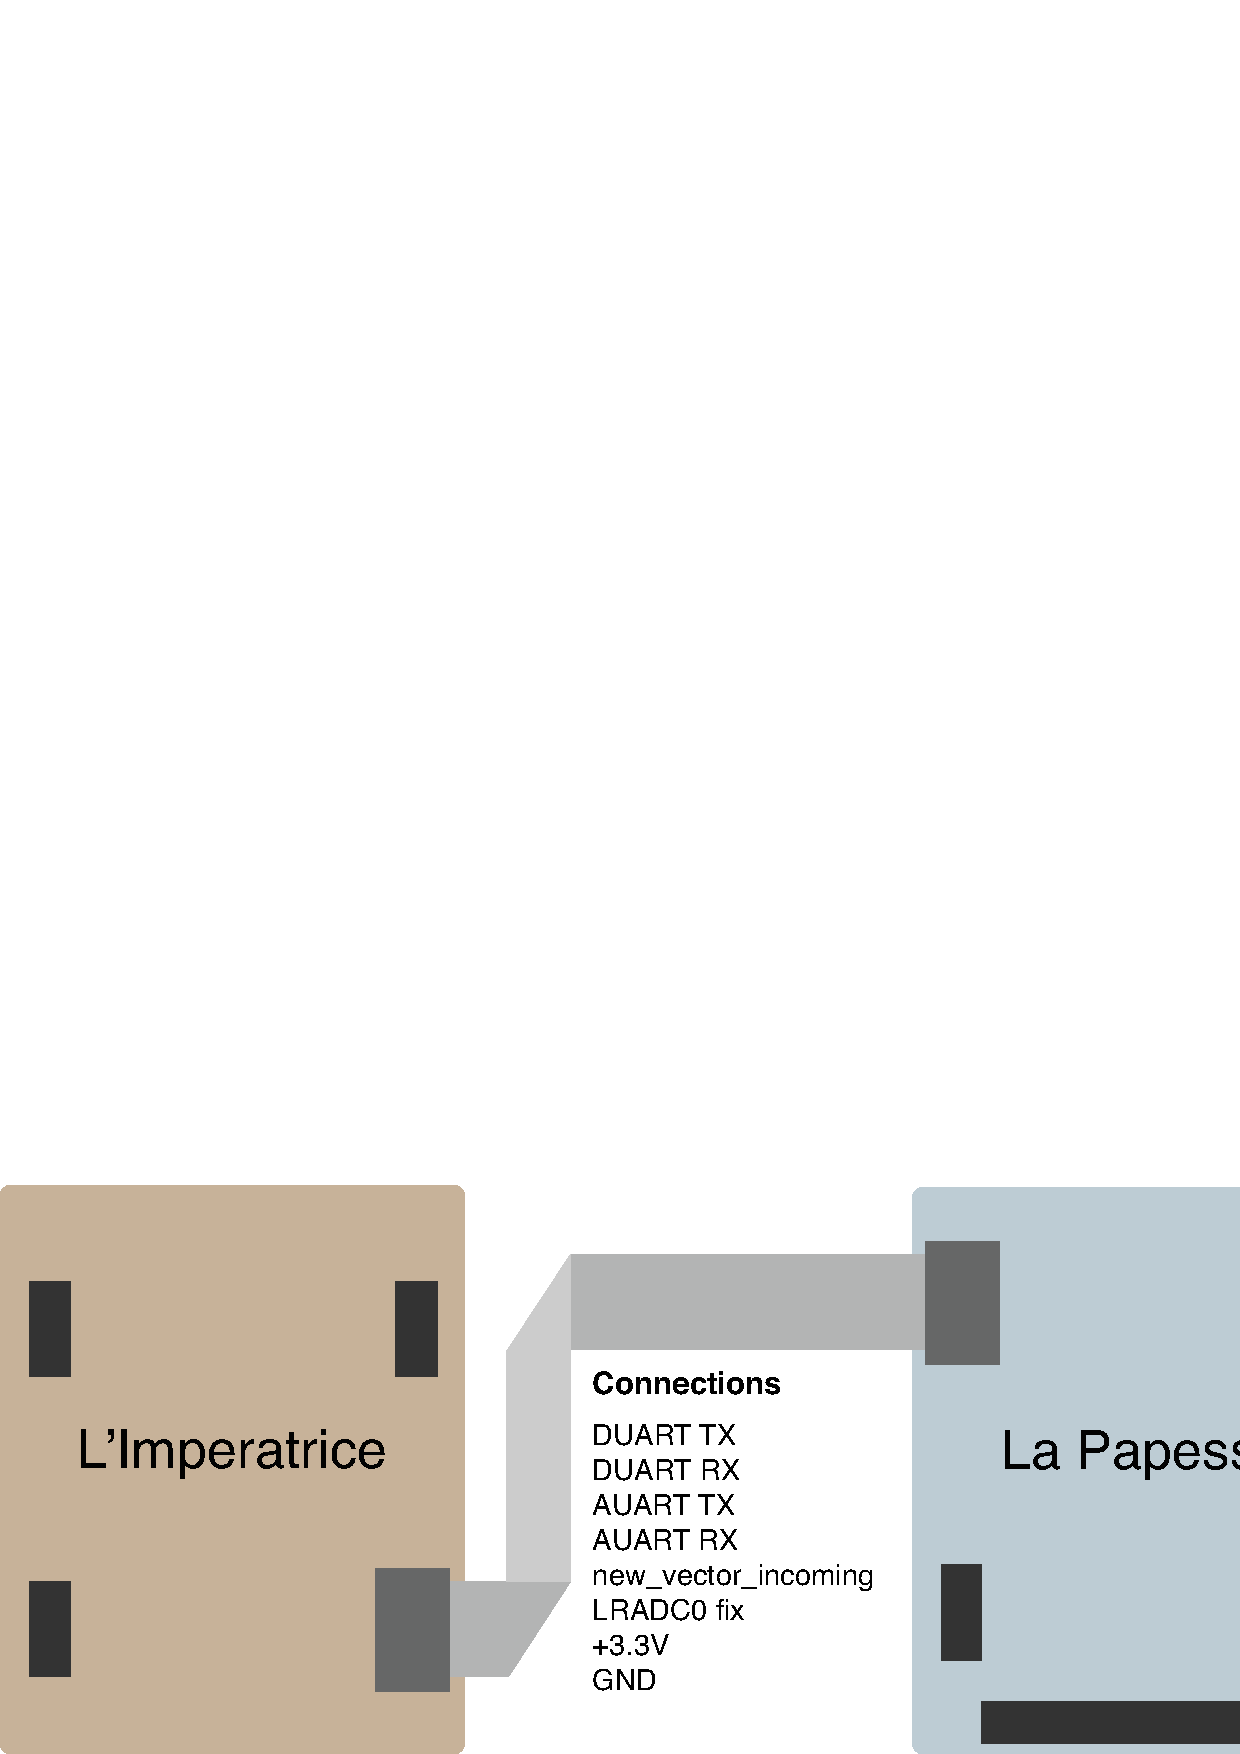
\includegraphics[width=\figwidth]{complete-system-overview.png}
		\end{center}
		\caption{Complete system overview}
		\label{fig:hlsystem}
	\end{figure}
% section system_overview (end)


\section{Number Format} % (fold)
\label{sec:number_format}
	% 16 bit numbers, scaling up and down
	% How were these chosen?
	Before beginning implementation of any part of the project, a number representation which would be appropriate for the FPGA had to be decided upon.  Firstly, it was recognised that using floating-point arithmetic on the FPGA would not be worth the effort, and therefore some form of fixed-point system was needed.  Further, the number magnitudes vary greatly between stages and parameters in the system.  In order to solve this problem, different scaling factors were used to bring most of the parameters to a similar magnitude.  

	The inputs and outputs of the Gaussian Distance Pipe, the module that performs the core calculation, are all signed 16-bit fixed point numbers, with varying scaling factors.  In particular, the $k$ parameter was generally larger than $x$, $mean$, and $omega$, and thus was scaled down.  The scaling factors were decided primarily by analysing the HMM models, to determine the largest and smallest numbers used.

	These decisions were influenced by Melnikoff \cite{melnikoff2003speech}, and the HTK, as they both use scaled 16-bit numbers to represent the parameters and scores.
% section number_format (end)


\section{La Papessa (The FPGA)} % (fold)
\label{sec:la_papessa_fpga}
	% The development environment used (Detailed documentation in Appendix)
	% GD Pipeline
	% SRAM
	% Controller
	% Normaliser pipeline
	% Communications

	The system on La Papessa performs these main tasks:
	\begin{itemize}
		\item Receives observation vectors from L'Imperatrice.
		\item Computes the score (Equation~\ref{eq:score_final}) of every senone in the model, with the given observation.
		\item Normalises the senone scores.
		\item Sends the scores back to L'Imperatrice.
	\end{itemize}

	\subsection{Top Level Module} % (fold)
	\label{sub:top_level_module}
		A simplified diagram of the top level module is given in Figure~\ref{fig:toplevel}, showing the main components of the system.  This module included the main controller logic, which essentially waited for a new observation vector, then cycled through the necessary operation states.  Figure~\ref{fig:topstatemachine} shows an ASM of this logic, and also outlines the main areas of the design that need explanation.

		The top level module is also responsible for handling access to the on-board SRAM chip, which several modules need to write or read from.  It essentially multiplexes the required signals, and leaves them floating (high impedance) when they are not needed.  The ``Debug signals'' shown in Figure~\ref{fig:toplevel} are a number of internal signals that are routed to output ports in order to facilitate hardware debugging.

		\begin{figure}[tb]
			\begin{center}
				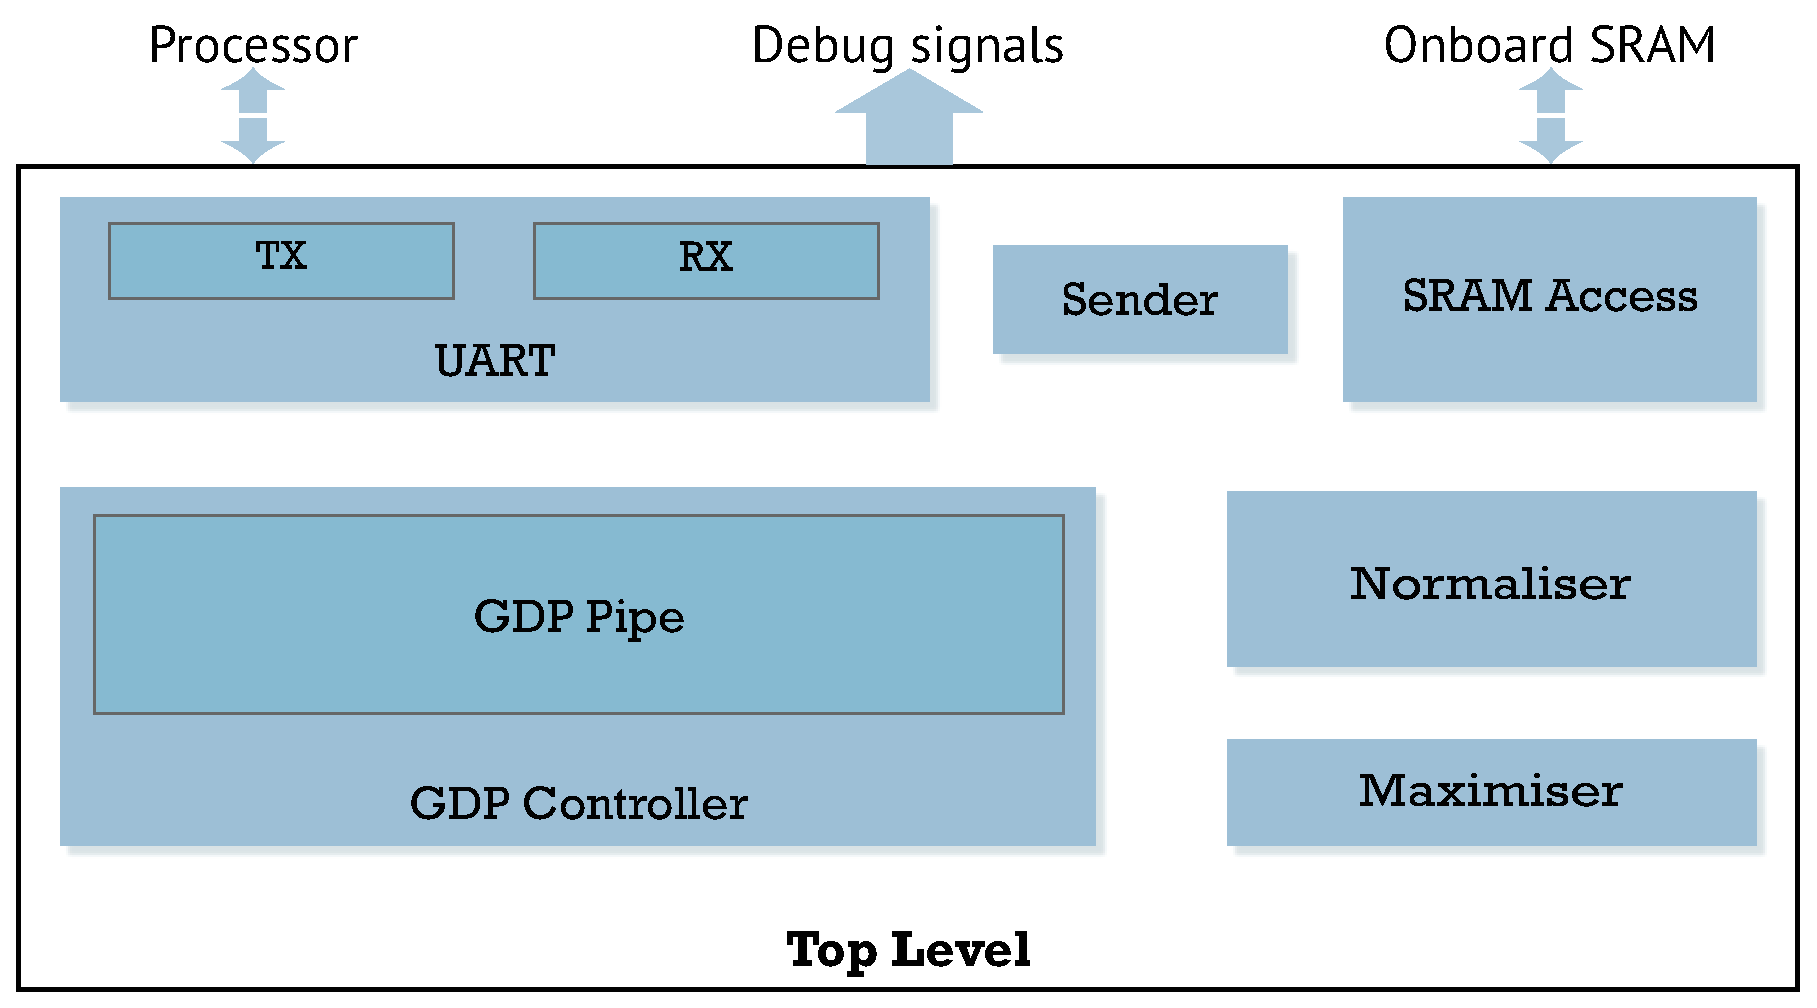
\includegraphics[width=\textwidth]{top_level}
			\end{center}
			\caption{Component diagram of the Top Level Module (Section~\ref{sub:top_level_module})}
			\label{fig:toplevel}
		\end{figure}

		\begin{figure}[tb]
			\begin{center}
				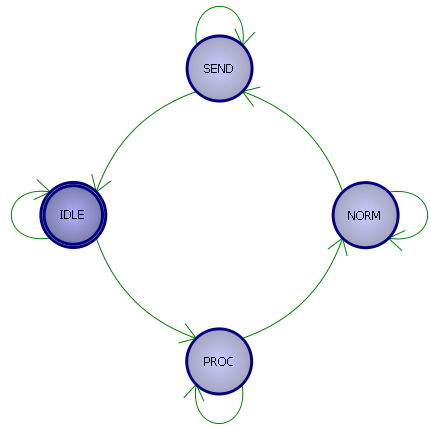
\includegraphics[width=0.6\textwidth]{TopLevel_asm}
			\end{center}
			\caption{ASM diagram of Top Level Module (Section~\ref{sub:top_level_module})}
			\label{fig:topstatemachine}
		\end{figure}
	% subsection top_level_module (end)

	\subsection{Gaussian Distance Pipeline} % (fold)
	\label{sub:gaussian_distance_pipeline}
		The Gaussian Distance Pipeline (GDP)\nomenclature{GDP}{Gaussian Distance Pipeline} is the core component of the system, and computes Equation~\ref{eq:score_final}.  It is a relatively simple 4-stage pipeline, with one stage for every step in the equation (subtract, square, scale, accumulate).  Although the gains from using a pipeline in this case are relatively small, it would be very useful if more complex models were used.  The Speech Silicon \cite{schuster2006speech} project had a substantially more complex GDP, as their senones have several Gaussian distributions that must be mixed to produce the final output distribution.  A block diagram of the GDP module is shown in Figure~\ref{fig:gdp_block}.  %TODO: describe the inputs etc...

		\begin{figure}[tb]
			\begin{center}
				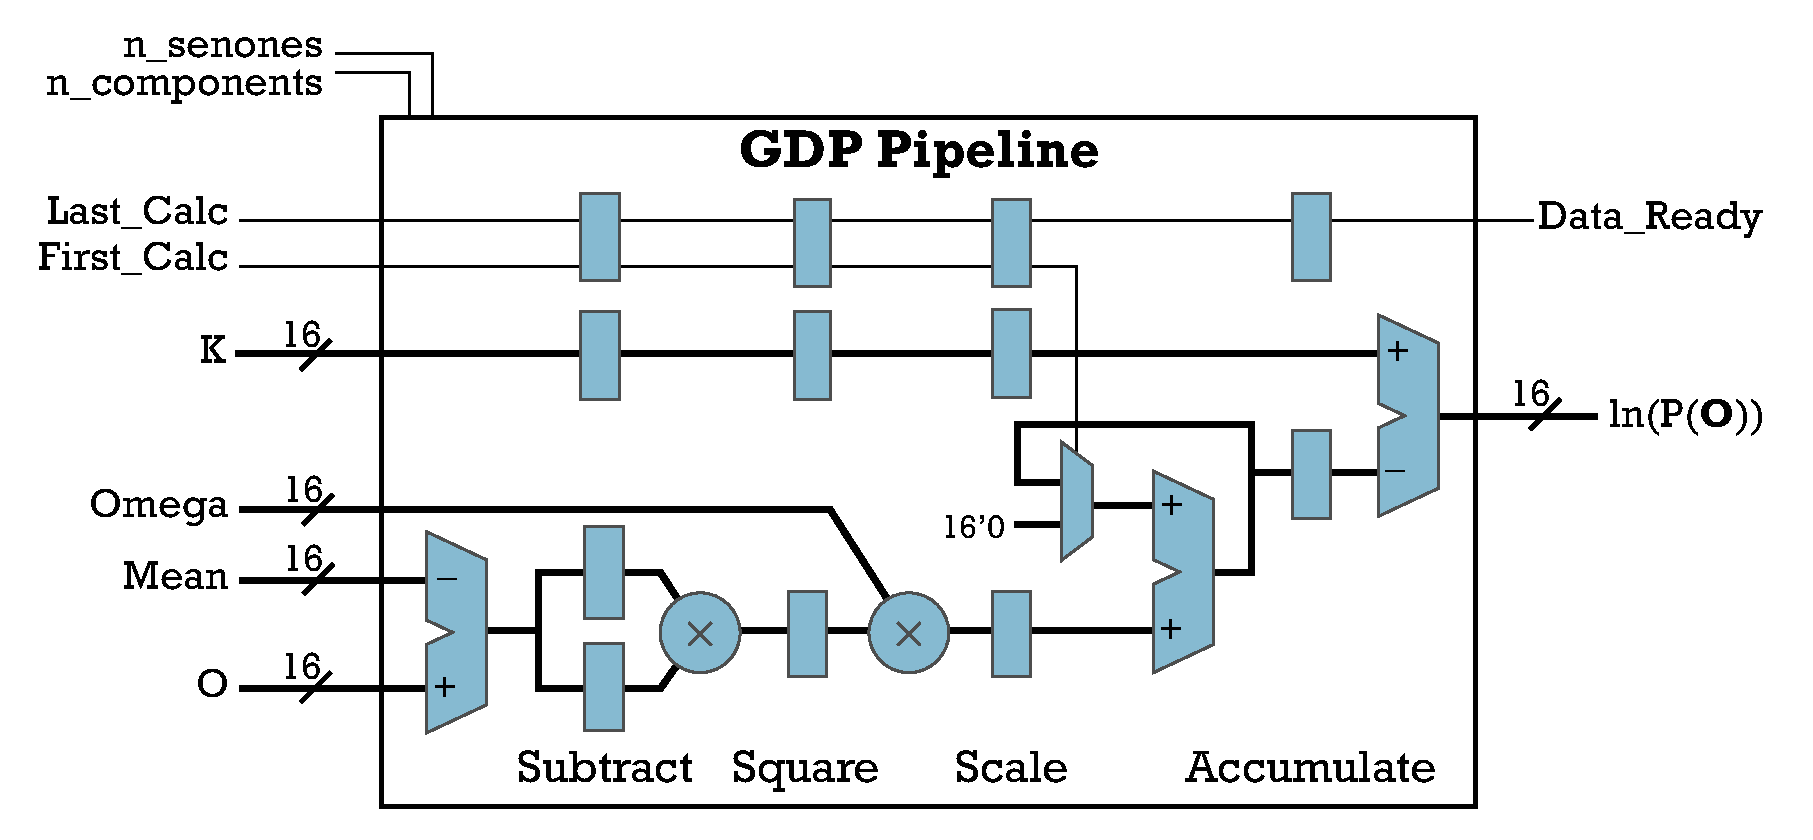
\includegraphics[width=\textwidth]{gdp_module_block}
			\end{center}
			\caption{Gaussian Distance Pipeline block diagram}
			\label{fig:gdp_block}
		\end{figure}

		In this module, `\texttt{n\_senones}' and `\texttt{n\_components}' are both parameter inputs, which determine the number of senones and the number of components per mean and variance in the model.  This allowed the design to be scaled down as size constraints became restrictive.

		The pipeline itself is a static object without much control logic, and thus requires a controller which sequentially uses it to score each senone in the model.  This controller is a simple state machine of only two states (\texttt{IDLE} and \texttt{LOAD\_GDP}), which begins feeding the pipe when a `\texttt{new\_vector\_available}' input flag is asserted.  This module is shown in Figure~\ref{fig:gdp_ctrl_block}.  A `\texttt{last\_senone}' output flag is asserted when the GDP produces the last senone score.  When the controller is in the \texttt{LOAD\_GDP} state, it essentially loops through the senones in the model, extracting their parameters and sending them to the GDP.  

		In order to facilitate the extraction and manipulation of senone parameters, a SystemVerilog structure was created, shown in Listing~\ref{lst:senonestr}. A SystemVerilog ROM module, connected to the controller, was populated with the senone parameters, stored in this structure.  Thus, when `\texttt{new\_vector\_available}' is asserted, the controller simply counts from 0 up to \texttt{n\_senones} (the number of senones in the model), and pulls the required parameters out of the ROM.

\begin{lstlisting}[style=customc, label=lst:senonestr, caption=Senone parameter data structure]
typedef struct packed {  /* num: typedef logic signed [15:0] num; */
  num k;
  num [n_components-1:0] omegas;
  num [n_components-1:0] means;
} senone_data;
\end{lstlisting}

		After asserting \texttt{new\_vector\_available}, and providing the relevant vector on the `\texttt{x}' input, the top level module will see  senone scores being sequentially produced, along with an index or ID which is unique to each senone.  The Top Level module is then responsible for storing the score in SRAM, and a ``Maximiser'' module registers the highest score seen.
		%TODO: show a multisim diagram of the normaliser??
		%TODO: where does it get its data from???
		\begin{figure}[tb]
			\begin{center}
				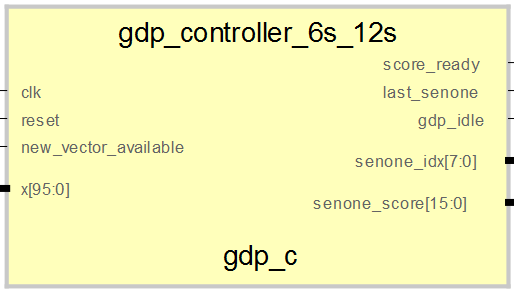
\includegraphics[width=\figwidth]{gdp_ctrl_block.png}
			\end{center}
			\caption{Gaussian Distance Pipe Controller block diagram}
			\label{fig:gdp_ctrl_block}
		\end{figure}
	% subsection gaussian_distance_pipeline (end)

	\subsection{Normalising Scores} % (fold)
	\label{sub:normaliser}
		The Speech Silicon architecture included a module which normalised the senones before they were used for decoding.  A very similar module is implemented here to perform the same normalisation.  The highest score is found while senones are being evaluated, and then this score is subtracted from all the final scores.  This causes the senone with the highest score to have a score of 0, which corresponds to a probability of 1 (the scores are log probabilities, see Section \ref{sub:senone_scoring}).
	% subsection normaliser (end)

	\subsection{SRAM} % (fold)
	\label{sub:onboard_sram}
		In order for the normaliser to access the senone scores, they must be stored somewhere as they are processed through the GDP.  One option would be to store them on the FPGA itself, where they would be accessible to all the modules.  However, this is impractical due to the potential size of an HMM model, and thus the large amount of RAM that would be required.  A better alternative would be to use external SRAM with low latency that is made accessible to whichever modules need it.

		Revision C of La Papessa board includes an on-board SRAM chip, which has an 8 bit data bus and 21 bit address bus, and was completely untested before this work.  In order to use it easily, a module was created primarily to interface the 8 bit data bus with the 16 bit number system used.  It's only operations are to write and read 16 bit values to the SRAM, and signal when it is ready or idle.  This is accomplished with the state machine shown in Figure~\ref{fig:sram_asm}.

		\begin{figure}[tb]
			\begin{center}
				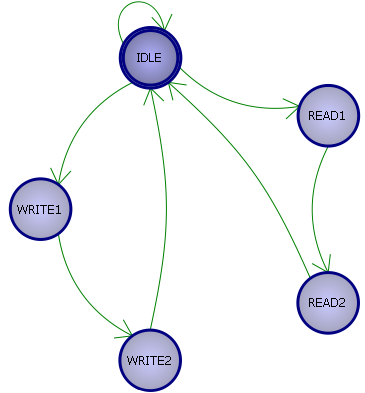
\includegraphics[width=0.6\textwidth]{SRAM_asm}
			\end{center}
			\caption{ASM of the SRAM access module (\ref{sub:onboard_sram})}
			\label{fig:sram_asm}
		\end{figure}
	% subsection onboard_sram (end)

	\subsection{Communications} % (fold)
	\label{sub:fpga_communications}
		The primary method of communication between the FPGA and processor is a standard UART bus, running at 115200 baud.  The communications module on the FPGA is essentially comprised of standard UART receive/transmit modules and a module that is wrapped around them to provide a higher level of data abstraction.  Because numbers are all 16 bits long in this system, and UART words are normally 8 bits, one of the wrapper purposes is to receive and transmit 16 bit numbers.  In addition, it is known beforehand that the FPGA should receive a certain number of bytes per observation vector.  This allows the UART module to wait until a 'packet' with that number of bytes has arrived, before signalling to the main controller that a new vector has arrived.  In this implementation, a buffer is simply filled up as new bytes arrive, and then is passed to the main controller when full.  However, it may happen that the UART module erroneously receives a byte, causing the buffer to be one byte fuller than it should be, and therefore causing the last byte of a new observation to be dropped.  In order to work around this, a `\texttt{new\_vector\_incoming}' flag is added, which will empty the buffer when asserted by the processor.  Another (possibly better way) of avoiding errors would be to automatically empty the buffer if new data is not received for a time-out period.  However, this is left as a possible future enhancement, as the \texttt{new\_vector\_incoming} flag is sufficient for now.

		The Baudticker module generates clock signals for the transmit and receive modules.  The transmit module requires a signal at approximately 115200Hz, but the receive module requires a signal at 8 times that frequency.  The receiver oversamples the input \texttt{rx} signal at this higher frequency, which enables it to detect and ignore signal glitches.  % TODO: finish this

		The Sender module is fairly simple in its operation -- it loops through all the senone scores stored in external SRAM and sends them over UART to the processor.
	% subsection fpga_communications (end)

% section la_papessa_fpga (end)


\section{L'Imperatrice (The processor)} % (fold)
\label{sec:l_imperatrice_processor}
	% GPIO
	% App UART
	% FFTW - compilation, LTIB, usage
	% LibMFCC
	% Various bits from HTK (liftering etc)
	% Makefile

	L'Imperatrice performs these main tasks:
	\begin{itemize}
		\item Read speech data from a WAV file.
		\item Pre-process -- pre-emphasise and window data, calculate FFT, calculate MFCCs, `Lifter' MFCCs.
		\item Convert MFCCs to the correct binary format.
		\item Send this observation vector to La Papessa.
		\item Receive and display scores.
	\end{itemize}

	% The most important task is the pre-processing -- Once this is done, it is a fairly simple matter to convert it to the correct 16-bit binary format, send the observation, and display the received scores.  

	\subsection{Pre-processing} % (fold)
	\label{sub:pre_processing}
		Instead of reading data in from a microphone, the system uses pre-recorded speech stored in WAV formatted audio files.  This method was chosen because it allows the pre-processing to be very easily tested, without worrying that the input data was changing.  In addition, it allowed the results to be compared with pre-processed data from other libraries, such as the HTK, in order to verify correct operation.

		The audio files were prepared specially, in a format that is simple to read and use.  The audio manipulation software `Audacity'\footnote{Audacity is available at \href{http://audacity.sourceforge.net/}{http://audacity.sourceforge.net/}, last checked April 2013.} was used to record and store speech as uncompressed (Microsoft) WAV files with unsigned 8-bit PCM encoding.  As Audacity does not support saving files with 8kHz sampling rates, the `sox'\footnote{SOX (Sound eXchange) is available at \href{http://sox.sourceforge.net/}{http://sox.sourceforge.net/}, last checked April 2013.} utility was used to downsample them from 48kHz to 8kHz.

		In pre-processing the data, an attempt was made to match the processes that the HTK used as closely as possible, thus making it easier to verify that the process works correctly.  Samples from the audio files are read in sequential blocks of between 80 and 200 samples, depending on the window size required.  These blocks are windowed with a Hamming window to remove discontinuities at the edges which could cause excess spectral noise.  The DFT is taken of this data, using the FFTW library, which had to be specially packaged and compiled for use in LTIB (See Appendix~\ref{apdx:compiling_fftw_for_ltib}).  Finally, the magnitude is taken, so that the spectral data is fully real and may be used to calculate Mel Frequency Cepstral Coefficients (MFCCs).  An external library (LibMFCC) was used for this purpose, due to its availability and the time constraints on the project.  The last operation, shown in Equation~\ref{eq:ceplifter}, is to perform Liftering\footnote{The name ``Liftering'' comes from the HTK book \cite{htkbook}} on each of the coefficients, where $L$ is a parameter.  This results in the cepstral coefficients having similar magnitudes \cite{htkbook}, which is particularly convenient when they must be represented with a 16-bit fixed-point number.
		\meq{ceplifter}{
			{c^{\prime}}_n
			= \left(1 + \frac{L}{2} sin \frac{\pi n}{L}\right) c_n
		}
	% subsection pre_processing (end)

	\subsection{GPIO and Application UART} % (fold)
	\label{sub:gpio_application_uart}
		In order to communicate with the FPGA, the processor required access to a serial port.  The ideal solution is the built-in Application UART port on the iMX23 chip, which only needs configuring.  In addition, access to GPIO from inside a C program was required to assert the \texttt{new\_vector\_incoming} signal.

		Both GPIO and Application UART must be enabled by selecting the relevant entry in the Kernel configuration menu at compile time (See Appendix~\ref{apdx:ltib_usage}).  Using the Application UART from a C program requires opening the serial port file (\texttt{/dev/ttySP1}, usually) and using the \texttt{termios.h} library to configure it correctly.  The options used to configure the serial port are shown in Listing~\ref{lst:serialconfig}.

\begin{lstlisting}[style=customc, label=lst:serialconfig, caption=Serial Port Configuration]
/* Set important serial port parameters: */
stty.c_cc[VMIN] = 0;                          // No blocking read
stty.c_cc[VTIME] = 1;                         // 0.1s: Max wait for data
stty.c_cflag = (stty.c_cflag & ~CSIZE) | CS8; // 8 bit chars
stty.c_iflag &= ~IGNBRK;                      // Ignore break commands
stty.c_lflag = 0;
stty.c_oflag = 0;
stty.c_iflag &= ~(IXON | IXOFF | IXANY);      // No flow ctrl
stty.c_cflag |= (CLOCAL | CREAD);             // enable receiver
stty.c_cflag &= ~(PARENB | PARODD);           // No parity
stty.c_cflag &= ~CSTOPB;                      // Send 1 stop bit
stty.c_cflag &= ~CRTSCTS;
\end{lstlisting}

		The GPIO is accessible in more than one way -- either through sysfs or via direct register access.  The kernel is configured to include the sysfs GPIO interface, which creates an entry under \texttt{/sys/class/gpio} that allows GPIO pins to be written and read as standard files.  Alternatively, the `Olinuxino' board project (which uses the same processor as L'Imperatrice) includes C code to directly write and read the GPIO registers as mapped memory\footnote{Accessible on the Olinuxino Github repository at \href{https://github.com/OLIMEX/OLINUXINO/}{https://github.com/OLIMEX/OLINUXINO/}}.  The project uses the second method, as it was straightforward to adapt the existing code for the purposes of the project.  In addition, direct memory access is far faster than the sysfs gpio interface; in tests, it was capable of switching frequencies up to 2MHz while the sysfs interface only managed about 200Hz.

	% subsection gpio_application_uart (end)

	% \subsection{Build process} % (fold)
	% \label{sub:build_process}
	% 	TODO??
	% % subsection build_process (end)

% section l_imperatrice (end)


\section{Support Software} % (fold)
\label{sec:support_software}
	A set of utilities were written in Common Lisp in order to facilitate and accelerate various parts of the project development.  Common Lisp was chosen due to its extreme power and flexibility, and because the IDE used, Emacs SLIME, is considered superior to any other.  In particular, these utilities helped with the following tasks (See Appendix~\ref{apdx:lisp_utils} for documentation):
	\begin{itemize}
		\item Parsing HMM definitions created by HTK, and extracting senone parameters
		\item SystemVerilog testbench generation
		\item Senone data file generation
		\item Verifying hardware functionality
		\item Number format conversion tasks
	\end{itemize}

	The HTK stores HMM definitions (along with transition matrices and senone definitions) in a human-readable plain-text Ascii file.  However, due to the very large model size, it was impractical to attempt to copy out parameters by hand.  For this reason, a parser was created that read an HMM definition file and stored the extracted data in a useful structure.  Another set of utilities was created to aid converting between floating point numbers and the custom fixed-point representations used.  

	Using these two sets of utilities, it was possible to automatically generate C header files and SystemVerilog modules containing the parameters, in a suitable format.  In addition, it became possible to easily and quickly generate testbenches to test the GDP with many different senones.
% section support_software (end)

% chapter system_design (end)  % 
%!TEX root = Main.tex
% System testing: words
\chapter{System Testing and Analysis} % (fold)
\label{cha:system_testing}

% Screenshots of data being sent and received (Logic)
% Timing analysis / diagrams

The testing methods and results are documented in this chapter.  The two primary blocks, described in the last chapter, were tested independently and then together, and will be presented here in the same manner.  A wide range of tools and techniques have been used to perform the testing, and to identify and fix errors encountered.

% Testing & things to document:
% x Testing methodology
% x GDP (software & hardware)
% x UART
% x SRAM (pre-tests, etc)
% x MFCCs
% Time of calculations, hardware vs software
% Full System - bus pirate, etc
% Hardware testing?? Current draw etc? .... Nah

\section{FPGA Design and Test Methodology} % (fold)
\label{sec:fpga_design_and_test_methodology}
	There were several phases of development, and thus testing, of this part of the design.  Initially, the full system was written and simulated in ModelSim, which supports SystemVerilog assertion based verification.  Each of the components of the design was built and tested separately, and then incrementally joined together and simulated as a whole.  Finally, the modules were tested in hardware -- first individually, and then as a full system.

	A set of testbenches were developed for use within ModelSim, which tested each of the modules used by the system.  Most of the modules were fairly simple to simulate and verify, as the expected behaviour is generally constant and determinate.  For example, verifying the UART clock generator was a case of instantiating it, asserting the enable signal, and verifying the frequency of the output signals.  However, some modules and their testbenches deserve extra attention, as special methods were used to test them.  In several areas, the benefits of using SystemVerilog become clear, as assertions greatly simplified the validation and testing process.

	Figure~\ref{fig:full_cycle} shows a simulation of the system performing a full cycle, from receiving an observation to sending back scores.
	\begin{figure}[tb]
		\begin{center}
			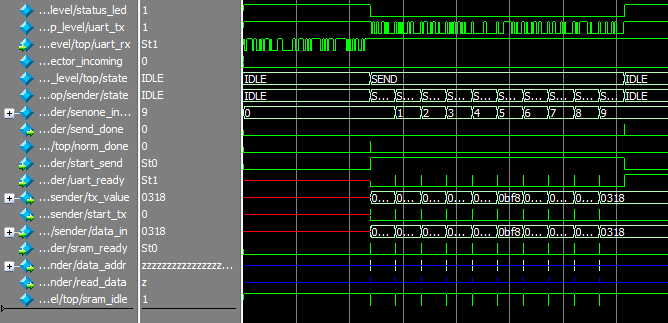
\includegraphics[width=\textwidth]{testbenches/full_cycle}
		\end{center}
		\caption{Simulation waveforms showing a full cycle of the top level state machine}
		\label{fig:full_cycle}
	\end{figure}
% section fpga_design_and_test_methodology (end)


\section{Gaussian Distance Calculation Block} % (fold)
\label{sec:gaussian_distance_calculation_testing}
	The Gaussian Distance Pipe was initially tested by creating a testbench which provided the sequence of inputs that the GDP required, and then asserted that the correct score was provided.  Figure~\ref{fig:test_gdp} shows the correct operation of this module, with a set of test data being used as inputs to the module.  The expected results were determined using the software GDP and the binary conversion software described in Section~\ref{sec:support_software}, thus confirming the validity of the results produced.

	\begin{figure}[tb]
		\begin{center}
			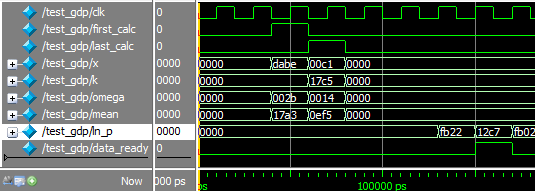
\includegraphics[width=\figwidth]{testbenches/gdp_wave}
		\end{center}
		\caption{GDP testbench waveform}
		\label{fig:test_gdp}
	\end{figure}
	
	The Gaussian Distance pipe controller testbench gives a new observation to the controller, and then watches as senone scores are produced by the module.  SystemVerilog assertions are used to check whether correct scores are arriving at the time they should.  However, in order to test a large number of different inputs (which would result in different score outputs), a set of software utilities were written to automatically generate the testbench code.  This software made use of the HMM definition parser and a software version of the GDP that had already been created.  This allowed a very large number of senones to be tested in a matter of minutes, and determine how well the GDP pipe was working.  Figure~\ref{fig:test_gdp_ctrl} shows the GDP Controller being tested.

	\begin{figure}[tb]
		\begin{center}
			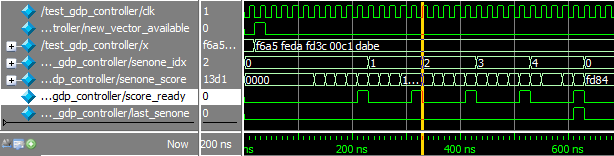
\includegraphics[width=\textwidth]{testbenches/gdp_ctrl_wave}
		\end{center}
		\caption{GDP Controller testbench waveform and error messages}
		\label{fig:test_gdp_ctrl}
	\end{figure}

	Being able to easily test many senones was important because the use of fixed-point arithmetic inevitably causes numerical errors that vary with the operations and numbers being used.  The GDP may produce the correct result for one set of inputs, but another set of inputs may produce an erroneous result that was caused by the fixed-point number not having high enough precision.  In fact, in most cases, the least significant bits of the result were wrong.  Because of this, it was important to determine the distribution of the error magnitudes, in order to decide whether the number format needed changing.  Automatic testbench generation made this far easier, as testbenches could be created which automatically displayed the senone scores that were wrong, and by how much.  The final system tolerated errors in the last 6 bits of the result, as this corresponds to less than 0.5\% of the total value.
	% TODO: talk about the error distribution??? I speak lots about how I found it (^) but don't actually say what the results were...


	From Figure~\ref{fig:test_gdp_ctrl}, it is also possible to observe the (ideal) time the GDP takes to calculate a score.  In this case (when \texttt{n\_components=5}), each senone takes 5 clock cycles (100ns with a 50MHz clock), after an initial pipeline loading delay.

	\subsection{Synthesis and Hardware Testing} % (fold)
	\label{sub:gdp_synthesis_and_hardware_testing}
		Unfortunately, due to the small size of the FPGA used, the initial synthesised design did not fit on it.  The full Voxforge model had over 7000 senones, and each observation had 25 parameters of 2 bytes each -- over 700kB of storage would be required for the full model.  As this far exceeds the resources available, the model size was reduced for the project.  The number of statistical parameters was reduced to 6, and only 12 senones were scored at once, bringing the FPGA slice usage to about 90\%.  % Confirmed.  Although at this %, may be clock skew!

		A variety of tools were used to repeatedly test the functionality of this hardware.  A Bus Pirate\footnote{Multi-purpose debugging tool that supports many different protocols.  See \href{http://dangerousprototypes.com/docs/Bus_Pirate}{http://dangerousprototypes.com/docs/Bus\_Pirate}} was used to communicate with the FPGA, which allows hexadecimal values to be easily sent and received over UART.  In order to debug the SystemVerilog, a large number of signals were routed to output pins, which were then monitored with a Saleae Logic analyser.
	% subsection gdp_synthesis_and_hardware_testing (end)
% section gaussian_distance_calculation_testing (end)


\section{UART Communications} % (fold)
\label{sec:uart_communications_testing}
	Simulating and testing the UART module was done by creating two instances of the module, and cross-connecting their RX and TX pins.  This allowed both transmit and receive to be tested, and confirmed correct operation.  An example of this testbench running is shown in Figure~\ref{fig:test_uart}.

	\begin{figure}[tb]
		\begin{center}
			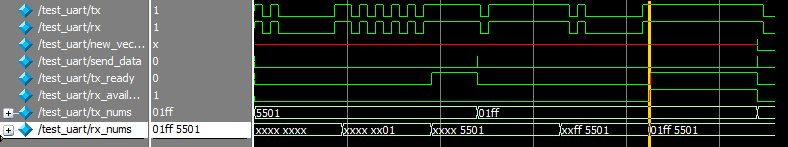
\includegraphics[width=\textwidth]{testbenches/uart_wave}
		\end{center}
		\caption{UART testbench waveform}
		\label{fig:test_uart}
	\end{figure}

	After simulation, the UART module was finally verified by programming the FPGA with the UART module, and a simple controller which echoed back whatever it received.  An FTDI USB to serial cable connected the FPGA to a computer, so that the setup could be confirmed to work with a real UART connection.  In addition, a Saleae Logic analyser was used to examine and ensure the absence of glitches in the UART signals generated by the FPGA.
% section uart_communications_testing (end)


\section{SRAM Access} % (fold)
\label{sec:sram_access_testing}
	A custom SystemVerilog module was designed in order to test writing and reading values to the SRAM chip, as it was a completely untested part of the board.  The module performed fairly basic operations, such as looping through a set of values, writing them to SRAM, and then reading them out again.  Debug information was displayed on the output pins, allowing the process to be monitored.  This confirmed that the chip worked as expected, and would be usable for the project.
% section sram_access_testing (end)


\section{Pre-Processing} % (fold)
\label{sec:pre_processing_testing}
	There were several different stages to the pre-processing, and these were tested individually.  First and foremost, the FFT code was tested by using input data containing known sinusoids.  The library used, FFTW, is well established and proven to work, and so the primary purpose here was to test the speed of the FFT.  It ran almost instantaneously (execution took 0.000000s, according to the Kernel time.h library), giving the correct results.

	The other major operation that required extensive testing was the MFCC calculation.  The other operations, pre-emphasis, windowing and liftering, are fairly straightforward mathematical operations that are easy to verify.  One of the desired properties of the system is that it would produce MFCCs that matched those produced by the HTK. Unfortunately, this was not quite achieved.  In most tests, the energy coefficient matched, but the others were relatively different.  This implies either that there is a limitation or problem with the MFCC library used, or that the HTK performs extra (or different) pre-processing.

	In addition, the library is very inefficient, causing the MFCCs to be produced relatively slowly.
% section pre_processing_testing (end)

\section{Software Based GDP Speed} % (fold)
\label{sec:software_based_gdp_speed_testing}
	The Gaussian Distance calculations were implemented in a C program in order to compare its performance with that of the FPGA.  It was found that the processor takes, on average, about 10$\mu s$ to calculate a single senone score -- about 100 times slower than the FPGA.  However, this version used double floating point precision, and thus is far more accurate than the FPGA.  Reducing the accuracy and using fixed-point values would definitely increase its speed.  % TODO!! Do this? It wouldn't be hard...
% section software_based_gdp_speed_testing (end)


% \section{Full system} % (fold)  % TODO
% \label{sec:full_system_testing}
% 	Once all the separate modules were tested and verified, the final task was to identify and eliminate the inevitable errors that occur once a design is integrated.

% % section full_system_testing (end)

% %!TEX root = Main.tex
% Project analysis: words
\chapter{Project Evaluation and Reflection} % (fold)
\label{cha:project_analysis}

This chapter presents an analysis of the final solution, evaluating its primary strengths and weaknesses, and the progress as a whole.

\section{Analysis of Solution} % (fold)
\label{sec:analysis_of_solution}

	\subsection{The FPGA} % (fold)
	\label{sub:analysis_the_fpga}
		The FPGA used was very small, and the full required design could not fit on it.  In particular, the size of the model had to be reduced, so that each Gaussian mean and variance had fewer than 25 components, and not all 7000 senones were processed.  However, what has been implemented is adequate to prove the concept, and demonstrate the advantages gained from using an FPGA.  In addition, it was known from the start that the full model would never fit, and so although this is a practical limitation, it does not make the project less worthwhile.

		Various benchmarks have been presented in the form of timing data.  It was shown that the FPGA was capable of calculating senone scores far faster than the traditional processor, albeit with an acceptable loss of accuracy.  This is similar to results achieved by Melnikoff \cite{melnikoff2003speech} and Speech Silicon \cite{schuster2006speech}, and supports the principle that custom-made hardware is faster than general purpose processors.  For real-time speech recognition, getting the senone scores as fast as possible is very important, as it allows more time for decoding tasks.  Thus, using an FPGA may be beneficial, especially in embedded systems.  It is possible to extrapolate, from the data gathered, the system speed when a larger model is implemented.  If the full model (7000 senones, 25 components) was used, the scores would be computed in about 3.5ms, leaving 6.5ms (of a 10ms window) for pre-processing and decoding (this excludes communications time).  If the embedded process was used to calculate the scores, it would take % TODO!!!! Recompile GDP-in-C with N_COMPS=25

		A big disadvantage of using an FPGA, in such a system, is the need to communicate to it.  The communication is an added step that adds time to the senone scoring process, and, if it is not fast enough, may render the use of an FPGA not worthwhile.  The implemented communication method (UART) is extremely slow and is the weakest point of the system, as is obvious in Figure~\ref{fig:full_cycle} which shows a complete cycle of the top level state machine.  Although it is not visible, the state machine goes through PROC and GDP, but these stages are far faster than the UART communication.  UART was used primarily for the ease of implementation, and because at this stage real-time operations are not required.  However, for this system to be realistically useful, a better communication method needs to be developed -- either a far faster serial bus or some form of hybrid serial-parallel connection.

		\begin{figure}[tb]
			\begin{center}
				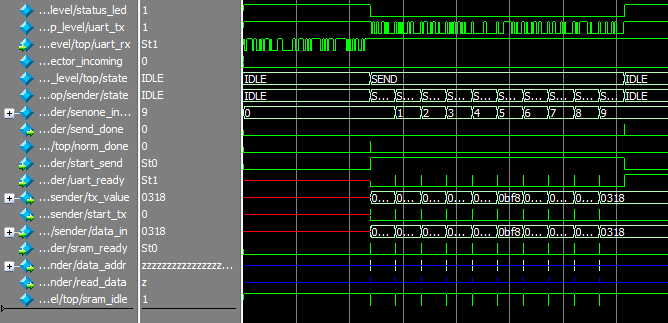
\includegraphics[width=\textwidth]{testbenches/full_cycle}
			\end{center}
			\caption{Simulation waveforms showing a full cycle of the top level state machine}
			\label{fig:full_cycle}
		\end{figure}

		% Additionally, the number format used caused the calculation accuracy to be reduced
	% subsection the_fpga (end)

	% Evaluate the speed - how long did each cycle take.  How much time was added by adding another component? or another senone? Extrapolate?

	\subsection{The Processor} % (fold)
	\label{sub:analysis_the_processor}
		The biggest problem, or limitation, with the current preprocessing system is the MFCC calculation step.  The external LibMFCC library is not optimised for the project's requirements at all, but it was convenient, and serves its purpose.  The HTK has a far faster implementation of this step, and could have been ported to the project code, had more time been available.

		However, what has been implemented is a good demonstration of the capabilities of this processor, and how it is capable of working with the FPGA.
	% subsection the_processor (end)


\section{Deviations from Original Goals} % (fold)
\label{sec:deviations_from_original_goals}
	Originally, while planning the project, the goal had been to implement a complete speech recognition system, from pre-processing to Viterbi decoding (see Appendix~\ref{apdx:brief}).  However, as more was learnt about the systems involved, it became clear that it was far too large a subject to attack in a single project.  Thus, the biggest change from initial plans was to narrow the project's focus down to a particular area of speech recognition.  However, with respect to the focussed goal, the results achieved are very satisfactoy.

	Development began by following the Gantt chart in Appendix~\ref{apdx:gantt_chart1}, which was also presented in the project Interim Report.  However, when building a software decoder proved to be far more time consuming than expected, the decision was made to change the focus, as mentioned above.  
	The remaining progress followed the Gantt chart in Appendix~\ref{apdx:gantt_chart2}\footnote{Both Gantt charts were created and modified using Gantter (http://app.gantter.com)}.  The majority of the design and implementation was completed in a timely manner, thus showing that the revised goals were more realistic.
% section deviations_from_original_goals (end)


% section analysis_of_solution (end)

% chapter project_analysis (end)

% chapter system_testing (end)         % Mostly done, needs expansion
%!TEX root = Main.tex
% Project analysis: words
\chapter{Project Evaluation and Reflection} % (fold)
\label{cha:project_analysis}

This chapter presents an analysis of the final solution, evaluating its primary strengths and weaknesses, and the progress as a whole.

\section{Analysis of Solution} % (fold)
\label{sec:analysis_of_solution}

	\subsection{The FPGA} % (fold)
	\label{sub:analysis_the_fpga}
		The FPGA used was very small, and the full required design could not fit on it.  In particular, the size of the model had to be reduced, so that each Gaussian mean and variance had fewer than 25 components, and not all 7000 senones were processed.  However, what has been implemented is adequate to prove the concept, and demonstrate the advantages gained from using an FPGA.  In addition, it was known from the start that the full model would never fit, and so although this is a practical limitation, it does not make the project less worthwhile.

		Various benchmarks have been presented in the form of timing data.  It was shown that the FPGA was capable of calculating senone scores far faster than the traditional processor, albeit with an acceptable loss of accuracy.  This is similar to results achieved by Melnikoff \cite{melnikoff2003speech} and Speech Silicon \cite{schuster2006speech}, and supports the principle that custom-made hardware is faster than general purpose processors.  For real-time speech recognition, getting the senone scores as fast as possible is very important, as it allows more time for decoding tasks.  Thus, using an FPGA may be beneficial, especially in embedded systems.  It is possible to extrapolate, from the data gathered, the system speed when a larger model is implemented.  If the full model (7000 senones, 25 components) was used, the scores would be computed in about 3.5ms, leaving 6.5ms (of a 10ms window) for pre-processing and decoding (this excludes communications time).  If the embedded process was used to calculate the scores, it would take % TODO!!!! Recompile GDP-in-C with N_COMPS=25

		A big disadvantage of using an FPGA, in such a system, is the need to communicate to it.  The communication is an added step that adds time to the senone scoring process, and, if it is not fast enough, may render the use of an FPGA not worthwhile.  The implemented communication method (UART) is extremely slow and is the weakest point of the system, as is obvious in Figure~\ref{fig:full_cycle} which shows a complete cycle of the top level state machine.  Although it is not visible, the state machine goes through PROC and GDP, but these stages are far faster than the UART communication.  UART was used primarily for the ease of implementation, and because at this stage real-time operations are not required.  However, for this system to be realistically useful, a better communication method needs to be developed -- either a far faster serial bus or some form of hybrid serial-parallel connection.

		\begin{figure}[tb]
			\begin{center}
				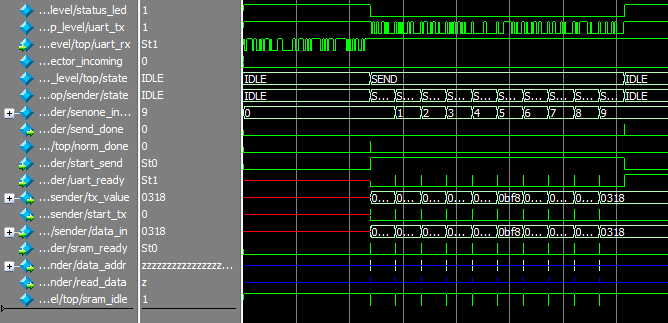
\includegraphics[width=\textwidth]{testbenches/full_cycle}
			\end{center}
			\caption{Simulation waveforms showing a full cycle of the top level state machine}
			\label{fig:full_cycle}
		\end{figure}

		% Additionally, the number format used caused the calculation accuracy to be reduced
	% subsection the_fpga (end)

	% Evaluate the speed - how long did each cycle take.  How much time was added by adding another component? or another senone? Extrapolate?

	\subsection{The Processor} % (fold)
	\label{sub:analysis_the_processor}
		The biggest problem, or limitation, with the current preprocessing system is the MFCC calculation step.  The external LibMFCC library is not optimised for the project's requirements at all, but it was convenient, and serves its purpose.  The HTK has a far faster implementation of this step, and could have been ported to the project code, had more time been available.

		However, what has been implemented is a good demonstration of the capabilities of this processor, and how it is capable of working with the FPGA.
	% subsection the_processor (end)


\section{Deviations from Original Goals} % (fold)
\label{sec:deviations_from_original_goals}
	Originally, while planning the project, the goal had been to implement a complete speech recognition system, from pre-processing to Viterbi decoding (see Appendix~\ref{apdx:brief}).  However, as more was learnt about the systems involved, it became clear that it was far too large a subject to attack in a single project.  Thus, the biggest change from initial plans was to narrow the project's focus down to a particular area of speech recognition.  However, with respect to the focussed goal, the results achieved are very satisfactoy.

	Development began by following the Gantt chart in Appendix~\ref{apdx:gantt_chart1}, which was also presented in the project Interim Report.  However, when building a software decoder proved to be far more time consuming than expected, the decision was made to change the focus, as mentioned above.  
	The remaining progress followed the Gantt chart in Appendix~\ref{apdx:gantt_chart2}\footnote{Both Gantt charts were created and modified using Gantter (http://app.gantter.com)}.  The majority of the design and implementation was completed in a timely manner, thus showing that the revised goals were more realistic.
% section deviations_from_original_goals (end)


% section analysis_of_solution (end)

% chapter project_analysis (end)        % 
%!TEX root = Main.tex
% Conclusions: 800 words
\chapter{Conclusions and Further Work} % (fold)
\label{cha:conclusions_and_future_work}

% Conclude....
% Re-state what was accomplished
% Personal gains - learnt loads, got to be the first doing something large with micro arcana, 
% Usefulness of result - someone interested in speech recognition, or 

This report presented a proof of concept system for carrying out speech recognition related operations on embedded hardware.  The system is built on two boards from the Micro Arcana family of development boards, and collectively performs two fundamental tasks:
\begin{itemize}
	\item Speech pre-processing, with Mel Frequency Cepstral Coefficients as the final observation vector.
	\item Scoring the states of HMMs in a speech model, given this observation vector.
\end{itemize}

A background of the relevant speech recognition theory was given, along with evaluations of various other techniques and approaches.  Descriptions and analyses of the completed design were presented, along with information on how it was tested.  In addition to the hardware based system, a multi-purpose software tool-kit was created that greatly helped during the design and testing stages of the project.

The principle goal was to design and implement part of an HMM based speech recognition system in embedded hardware, in order to evaluate and learn about such a system.  This has been fairly successful; the conclusions are given below.
% It was not intended to be used as a real recogniser, but rather to broaden the author's knowledge and experience, and provide a platform on which embedded speech recognition may be researched further.  
  % TODO: clean this paragraph up...


\section{Usefulness of Results} % (fold)
\label{sec:usefulness}
	Due to size limitations of the FPGA, it was not possible to use a complete HMM speech model with the implemented system.  However, the intention was never to build something that was usable with such a model, but rather to attempt to judge the usefulness of an FPGA in this situation.  With the results achieved it was possible to estimate the relationship between the system speed and model size, and thus show that the FPGA was capable of producing results faster than a traditional processor.

	Furthermore, this project is a valuable example of how two of the Micro Arcana family may be connected and used in a practical setting.  Some of the problems encountered are certainly not unique to this design, and therefore the solutions presented may be helpful in other projects.

	As a development platform, there is potential for further investigation into embedded speech recognition using the two systems built here.  Indeed, there are several different aspects of the design that may be expanded upon or improved, as described in the further work section.  This is not a failing of the current project -- speech recognition is such a large and complex area that only a small part of it could possibly be implemented in the time available.
% section usefulness (end)


\section{Future Work} % (fold)
\label{sec:future_work}
	There are many possibilities for developing this project further -- either by improving the system already built, or implementing other speech recognition tasks such as decoding.  With the system in its current state, there are a few areas that may be interesting to investigate.

	Primarily due to time constraints, the Mel Frequency Cepstral Coefficients were computed using an existing library (LibMFCC).  However, LibMFCC is extremely slow, and should definitely be optimised.  In addition, it would be very beneficial if the pre-processing generated the same MFCCs as those generated by the HTK.  This would require an in-depth analysis of the HTK system in order to determine the exact sequence of operations that are performed.

	Communications between the boards needs improvement before the system can be considered realistically usable.  Better communications would need to be far faster, and possibly include features such as error-checking, hand-shaking, and control sequences.  Designing a better communications method between two of the Micro Arcana boards would be an interesting project, due to the size and speed constraints of the family.

	This project only implemented the first stages of a speech recognition engine, and did not at all focus on tasks such as decoding or language modelling.  However, it provides an environment where these systems may be implemented and used.  There is huge potential for further work that could focus on any one of these areas.
% section future_work (end)


% \section{Personal Gains} % (fold)
% \label{sec:personal_gains}
% 	As the author is still exploring the vast world of electronic engineering, one of the attractions of this project was its diversity and complexity.  The project involved several different areas of electronics, including digital systems design, complex algorithms and optimisation, embedded Linux programming, and hardware testing.  Completing this project, with all the different activities involved, was personally satisfying, especially as it involved working with hardware that had never been used in this manner before.

% 	A sense of accomplishment followed completion of the system implementation, as it represented the union of many different technologies and techniques, useful from a educatory point of view, as well as being an interesting and challenging project.
	% I gained lots of experience with complex algorithms, digital design,
	% Even though I did not implement the more complex algorithms, it was interesting learning about them, and how they work.
	% This is the largest digital system I have ever built, and I have never interfaced an FPGA with a C program.  I have never used an embedded Linux board that was so undeveloped, and I have never
% section personal_gains (end)

% chapter conclusions_and_future_work (end)     % Mostly done

%% ---------------------------------------------------------------------------%
\bibliographystyle{plainnat}  % TODO: fix ecs bib style...
\dobib{../citations-ALL}

\appendices
%!TEX root = ../Main.tex
% Appendices Index

% Needed in Appendices:
%----------------------
%
% Detailed Doc of development environment for La Papessa and L'Imperatrice
% Detail how to build FFTW for LTIB
%
% Scripts and info for Voxforge model creation / adaption
%
% Project Brief

\newcommand{\includeA}[1] { \include{Appendices/#1} }

\includeA{Brief} % done
\includeA{ProjMan} % done

\includeA{DevEnv} % needs finishing
\includeA{Voxforge} % done
\includeA{LispUtils} % proof read

\includeA{ArchiveTree}

%% ---------------------------------------------------------------------------%
\end{document}
